\section{Simple Simulator}
\label{sec:simple-simulator}
% TODO: Say we can load pgm maps from ROS 2
The simple simulator was developed to enable rapid testing and debugging of robot swarm behavior in a controlled 2D environment. It simulates multiple robots operating in a discretized world, rendering them as circles with their respective IDs displayed at their centers. The simulator advances in discrete time steps at 60 updates per simulated second and executes in a multi-threaded fashion to maintain performance across large robot groups.\\

The simulator supports loading map layouts from ROS 2-compatible \texttt{.pgm} files, allowing it to closely mirror environments used in the 3D Gazebo simulations. This compatibility facilitates seamless testing of behaviors across both simulation platforms.

\Cref{fig:simple-sim-interface} shows the graphical user interface of the simulator, displaying a scenario where three robots are performing a coordinated search in the left region of the map.

\begin{figure}[H]
    \begin{center}
        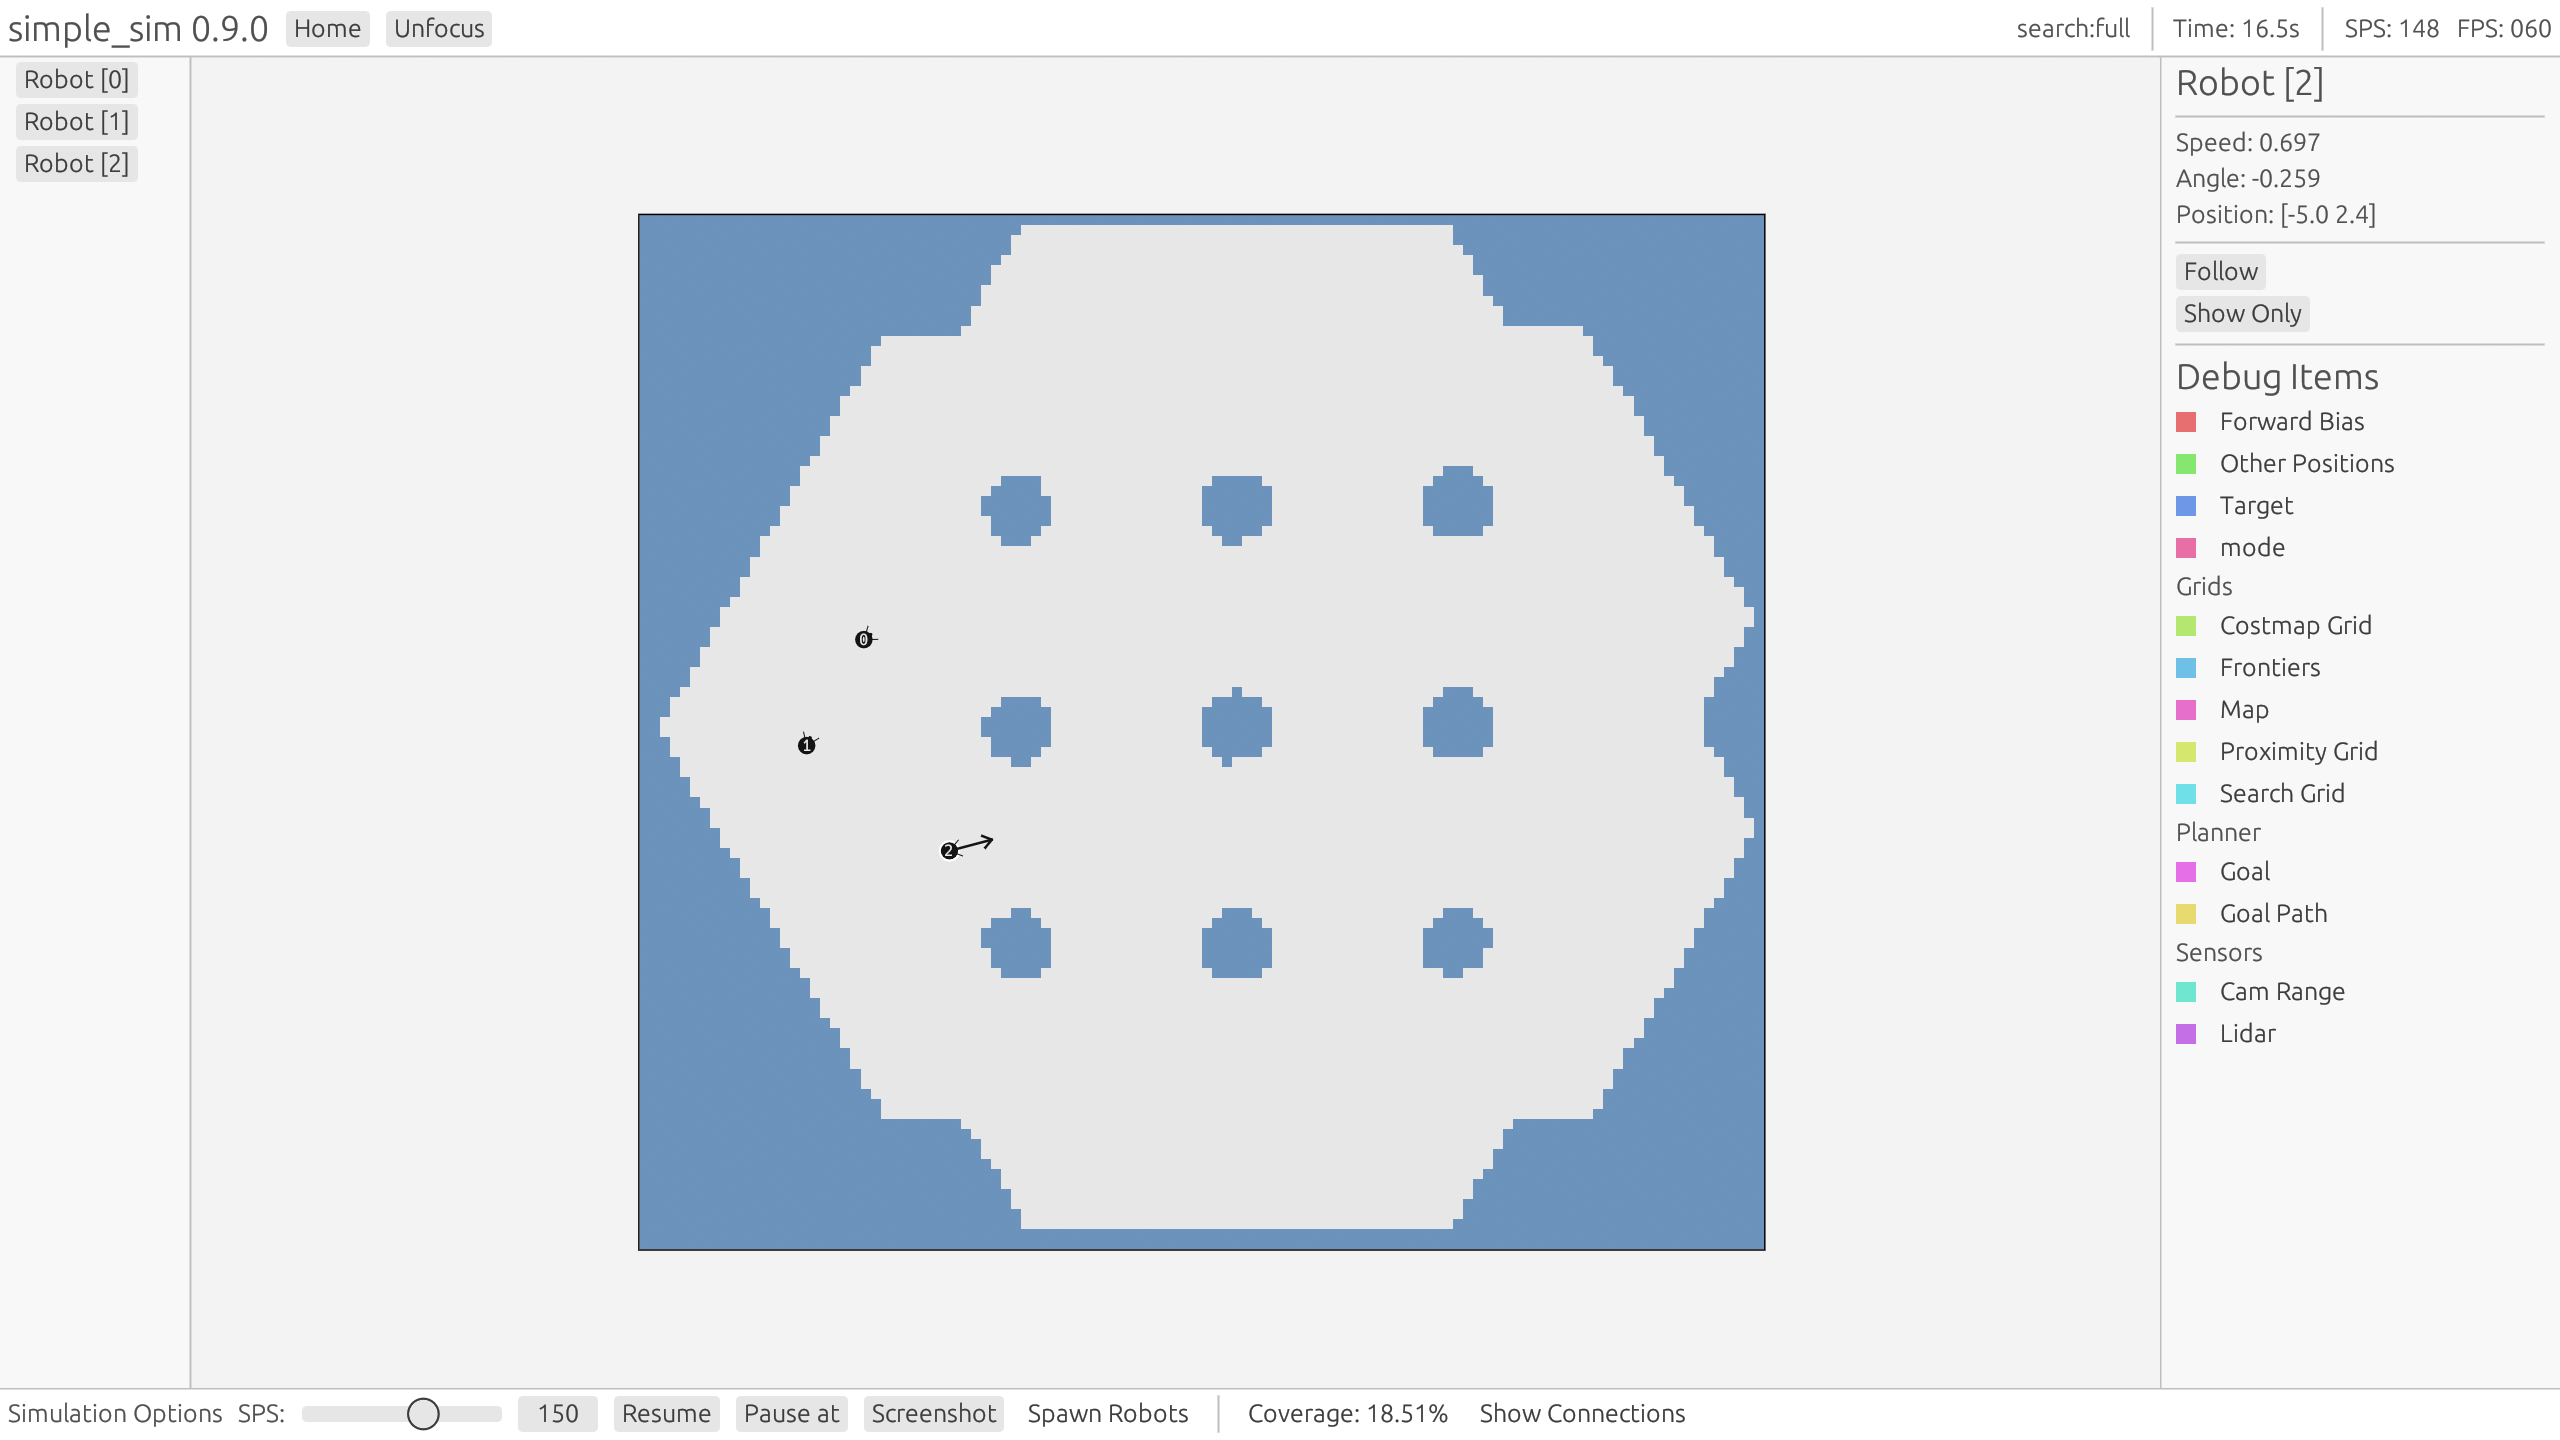
\includegraphics[width=0.95\textwidth]{figures/screenshots/simple-sim-gui.png}
    \end{center}
    \caption{Simple simulator interface showing three robots operating in a shared environment.}
    \label{fig:simple-sim-interface}
\end{figure}

% TODO: ray-marching cite
\subsection{Sensor Approximation}
To run behaviors, each robot requires input from three sources: pose, LiDAR, and camera data. The pose is set directly by the simulator and requires no approximation. However, both LiDAR and camera inputs are simulated using ray marching techniques \cite{raymarching}, a lightweight yet effective method for approximating line-of-sight sensor data in a 2D grid world.

LiDAR is simulated by emitting a series of radial rays from the robot's position at fixed angular intervals. Each ray is advanced incrementally until it intersects with an obstacle in the environment. The resulting distance data mimics real-world LiDAR output and is illustrated in \cref{fig:lidar-approximation}.

The camera simulation follows a similar ray-marching procedure but is constrained to a defined field of view, replicating the properties of the Turtlebot 4’s camera. Rather than applying a full object detection algorithm, the camera rays directly infer object identity upon intersection, allowing simplified yet functional input for the behavior algorithms.

% TODO: Maybe better colors for camera and lidar?
\begin{figure}
    \centering
    \begin{subfigure}[b]{0.45\textwidth}
        \centering
        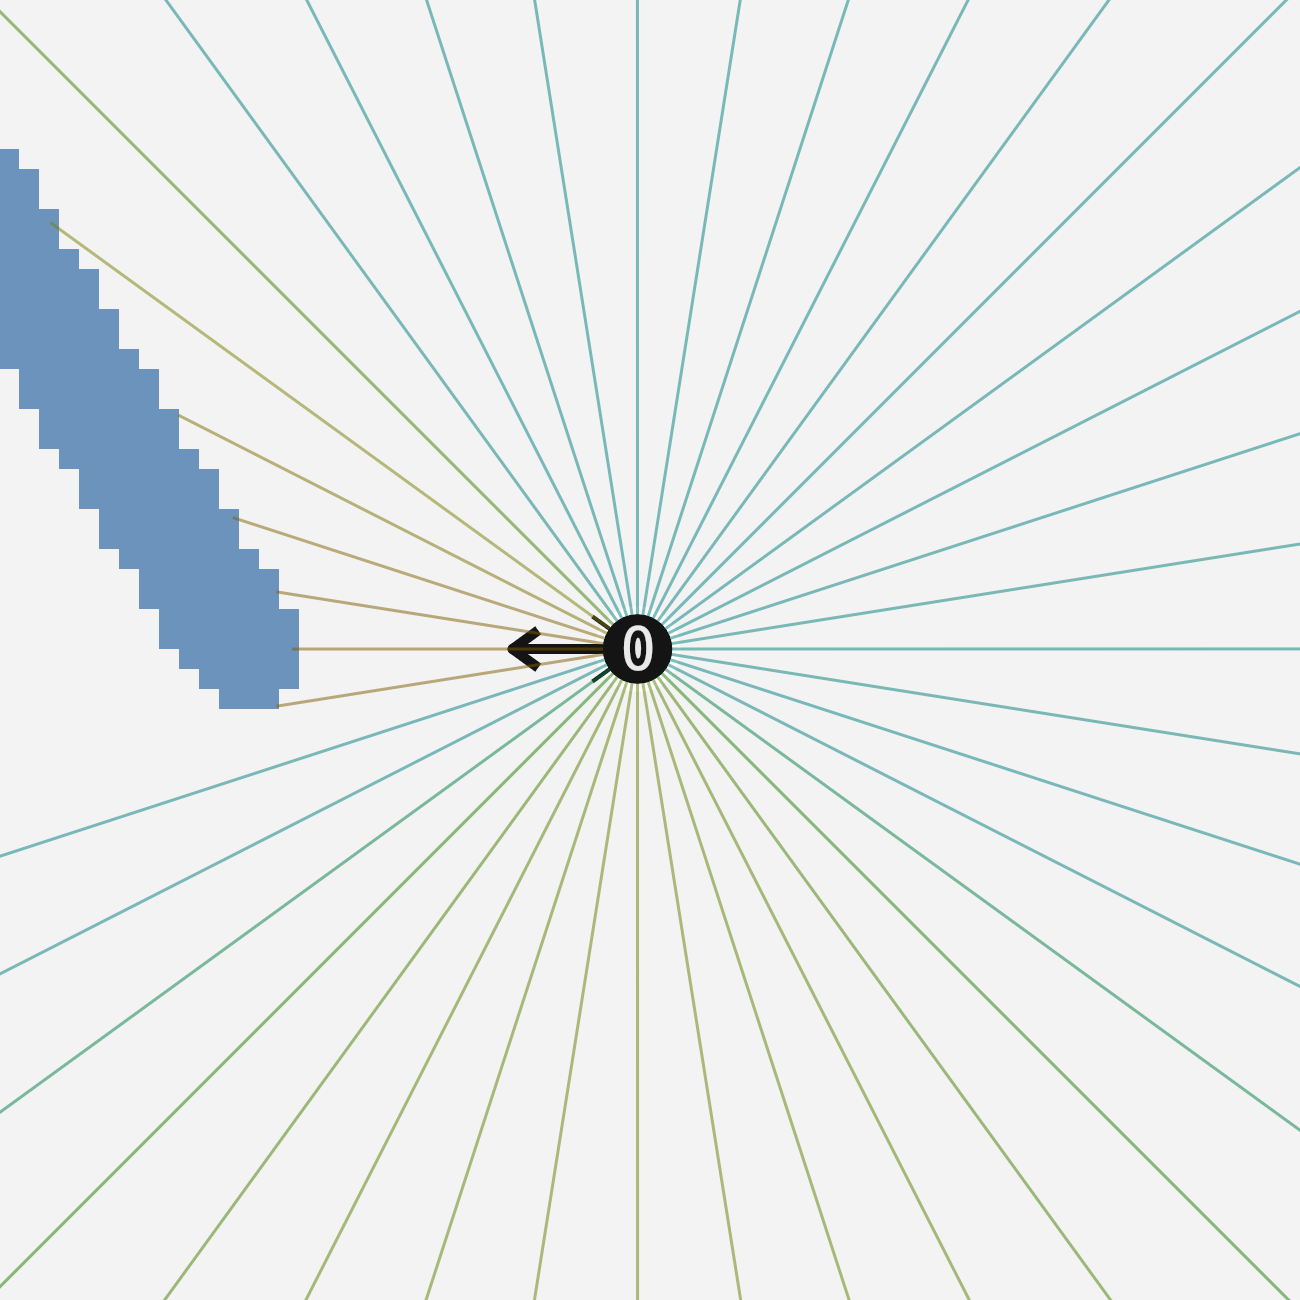
\includegraphics[width=\textwidth]{figures/screenshots/simple-lidar.png}
        \caption{LiDAR approximation}
        \label{fig:lidar-approximation}
    \end{subfigure}
    \hfill
    \begin{subfigure}[b]{0.45\textwidth}
        \centering
        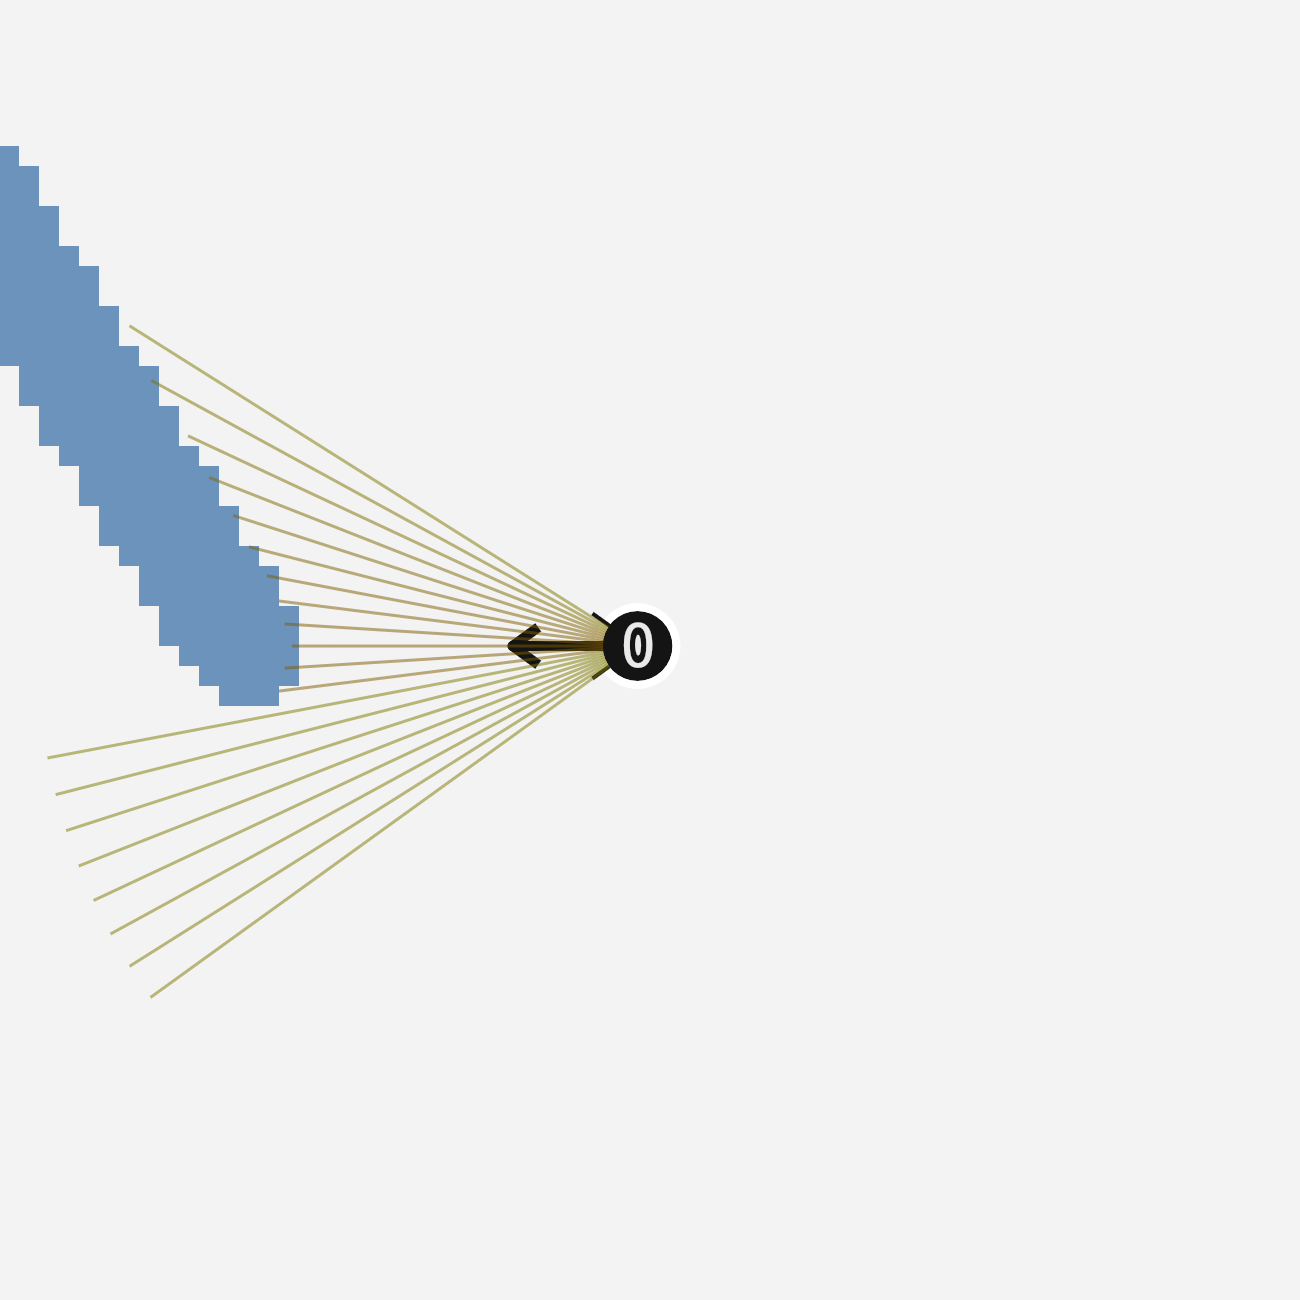
\includegraphics[width=\textwidth]{figures/screenshots/simple-camera.png}
        \caption{Camera approximation}
        \label{fig:camera-approximation}
    \end{subfigure}
    \caption{Sensor input approximation in the simple simulator.}
    \label{fig:sensor-approximation}
\end{figure}

\subsection{Debugging}
To facilitate development and validation, the simple simulator supports real-time debugging of both robot behavior and internal state. The \texttt{botbrain} library exposes a debugging interface known as \texttt{Debug Soup}, which allows behavior modules to annotate the simulation with structured debugging data. These debug items—such as occupancy grids, path vectors, target points, and internal decision states—can be visualized in both \texttt{simple\_sim} and ROS 2 via RViz2. The debug item in \texttt{simple\_sim} can be seen on the right side in \cref{fig:simple-sim-interface}.
This significantly accelerates the development process and helps in interpreting the emergent behavior of the swarm.

\subsection{Library}
The simulator architecture is built around the shared \texttt{botbrain} behavior library, which encapsulates each robot’s internal state and provides a standardized interface for behavior control. This modular design allows the same behavior code to be executed seamlessly in both the lightweight \texttt{simple\_sim} environment and the more realistic Gazebo/ROS~2 simulation without requiring any code changes.

By decoupling the behavior logic from the underlying simulation platform, the system supports consistent benchmarking and fair comparisons between algorithms. This separation also promotes cleaner, more testable, and reusable code, making it easier to iterate on behaviors and evaluate improvements.\\

The \texttt{simple\_sim} simulator itself is also implemented as a reusable library. In addition to running with a graphical user interface, it can be executed in headless mode—without visualization—for fast batch execution. This is particularly useful when collecting performance metrics, generating plots, or running reinforcement learning experiments where a large number of episodes must be simulated efficiently.

Moreover, the headless mode enables integration with external scripts or training pipelines, allowing behaviors to be evaluated or learned in a fully automated manner. This versatility makes \texttt{simple\_sim} an effective tool for both development and research use cases.

% TODO: Should this be here?
\subsection{Performance} 
The simple simulator is designed to be lightweight and performant. It supports deterministic execution, enabling reproducible tests for debugging and reinforcement learning. Simulation speed can be accelerated beyond real time, depending on CPU capacity and the number of robots simulated.

Multi-threading is used to parallelize sensor simulation and robot state updates, allowing the system to scale to larger swarms. In practical testing, the simulator is capable of running over 30 to 50 robots in real time on a standard desktop CPU depending on the behavior. Because the environment is purely 2D and avoids expensive physics calculations, the performance overhead is minimal compared to full 3D simulation.

This high-performance execution makes the simulator well-suited for training deep reinforcement learning agents, where a large number of episodes must be executed within a reasonable timeframe.
